% =====================================================================
%  Dissertation Progress Report — Milestones 1 and 2
%  Compile: pdflatex twice. Overleaf-ready, no external files.
% =====================================================================
\documentclass[11pt,a4paper]{article}

\usepackage[margin=2.3cm]{geometry}
\usepackage[T1]{fontenc}
\IfFileExists{lmodern.sty}{\usepackage{lmodern}}{}
\usepackage{booktabs}
\usepackage{array}
\usepackage{xcolor}
\usepackage{listings}
\usepackage{graphicx}
\usepackage{tikz}
\usepackage{caption}
\usepackage{enumitem}
\usepackage{amsmath}
\usepackage[hidelinks]{hyperref}
\usetikzlibrary{shapes.geometric, arrows.meta, positioning, fit, backgrounds, calc}

\definecolor{navy}{RGB}{18,42,86}
\definecolor{gold}{RGB}{184,138,40}
\definecolor{softgrey}{RGB}{242,243,245}
\definecolor{midgrey}{RGB}{120,126,134}
\definecolor{good}{RGB}{22,110,72}
\definecolor{bad}{RGB}{158,42,42}
\definecolor{codebg}{RGB}{248,248,250}

\lstdefinestyle{py}{
  language=Python, basicstyle=\ttfamily\scriptsize,
  keywordstyle=\color{navy}\bfseries, stringstyle=\color{good},
  commentstyle=\color{midgrey}\itshape, backgroundcolor=\color{codebg},
  frame=leftline, framerule=1.2pt, rulecolor=\color{gold},
  xleftmargin=8pt, framexleftmargin=6pt, breaklines=true,
  showstringspaces=false, aboveskip=5pt, belowskip=5pt,
}
\lstset{style=py}

\usepackage{titlesec}
\titleformat{\section}{\normalfont\large\bfseries\color{navy}}{\thesection}{0.6em}{}
\titleformat{\subsection}{\normalfont\normalsize\bfseries\color{navy}}{\thesubsection}{0.6em}{}
\setlength{\parskip}{0.42em}
\setlength{\parindent}{0pt}

\newcommand{\up}[1]{\textcolor{good}{\textbf{#1}}}
\newcommand{\down}[1]{\textcolor{bad}{\textbf{#1}}}

\begin{document}

% ---------------------------------------------------------------- title
\begin{center}
{\LARGE\bfseries\color{navy} Spatial Mental Modeling from Limited Views}\\[4pt]
{\large Dissertation Progress Report~---~Milestones 1--3}\\[10pt]
{\large\bfseries Reproducing ViperGPT without Codex:}\\[2pt]
{\large\bfseries a Prompt-Specification Gap and a Depth-Reasoning Gap}\\[13pt]
\begin{tabular}{rl}
\textbf{Student} & MD Humayun \\
\textbf{Supervisor} & Dr.\ M.A.\ Zaveri \\
\textbf{Programme} & M.Tech CSE (Information Security \& Privacy), SVNIT Surat \\
\textbf{Date} & 16 August 2026 \\
\textbf{Repository} & \texttt{mdhumayun7/Vipergpt}, tag \texttt{m3-final} \\
\end{tabular}
\end{center}
\vspace{4pt}\hrule\vspace{9pt}

\begin{center}\begin{minipage}{0.93\textwidth}\small
\textbf{Summary.}\; ViperGPT (Sur\'is et al., ICCV 2023) answers visual queries by
prompting a code LLM to emit a Python program over vision modules. Its generator,
Codex, has been retired, so every present-day reproduction must substitute an
open-weights model. We rebuilt the pipeline end to end on an H100 cluster and report
two results. \emph{First}, the released prompt never states that a grounding program
must return an \texttt{ImagePatch}; with Qwen2.5-Coder-7B this makes \down{98.8\%} of
programs task-invalid and yields \down{0.00\%} accuracy on RefCOCO. Adding a
return-type contract and two exemplars gives \up{39.20\%} (RefCOCO) and \up{31.80\%}
(RefCOCO+). \emph{Second}, having fixed that, accuracy splits sharply by the kind of
spatial language: 2D image-plane queries reach 35.29\%, while depth and relational
queries reach \down{6.38\%}. A scale sweep shows this is not a capacity problem ---
across 1.5B, 7B and 32B generators, non-spatial accuracy rises 33.65 $\to$ 48.82
while spatial accuracy is flat at 34.95 / 35.29 / 34.95. \emph{Third}, adding depth-ordering
primitives to the API raises depth-query accuracy from 4.26\% to \up{21.28\%}
(5$\times$) --- but only once the prompt also states \emph{when} they apply. Given the
primitives unconditionally the generator over-applies them and non-spatial accuracy
falls 10 points; given a routing rule it improves every subset simultaneously, taking
RefCOCO from 39.20\% to \up{42.00\%}.
\end{minipage}\end{center}
\vspace{6pt}

% =====================================================================
\section{Pipeline and what was built}

\begin{figure}[htbp]
\centering
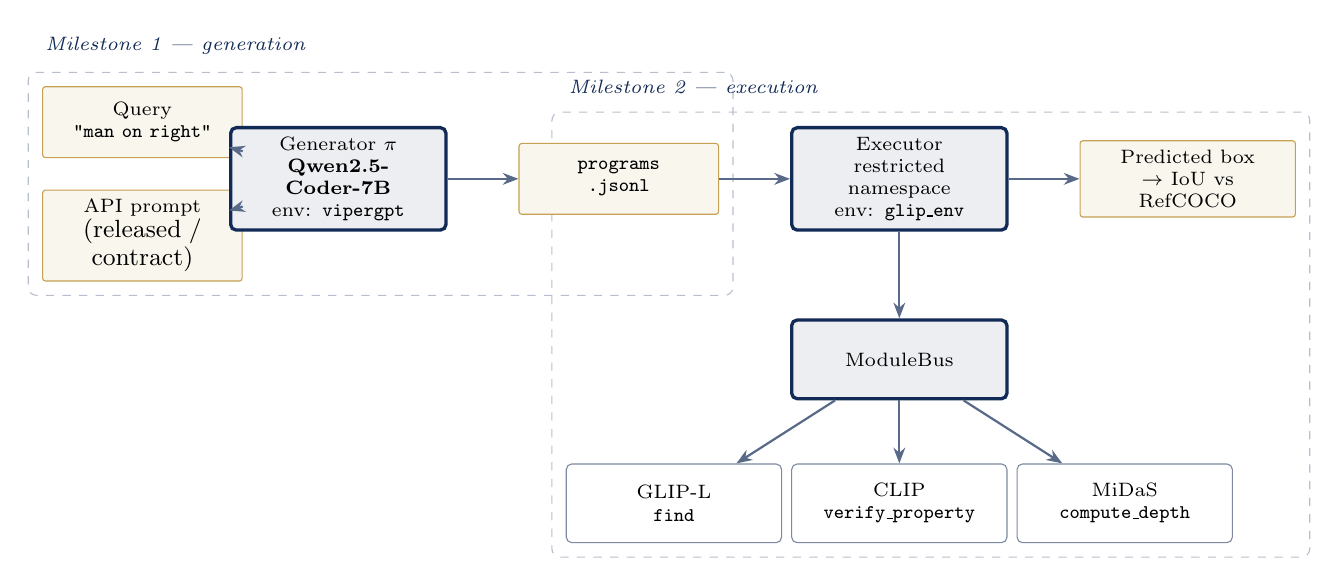
\begin{tikzpicture}[
  node distance=7mm,
  box/.style={rectangle, rounded corners=2pt, draw=navy!55, fill=white,
              text width=25mm, align=center, minimum height=10mm, font=\scriptsize},
  act/.style={box, fill=navy!8, draw=navy, very thick},
  data/.style={rectangle, rounded corners=1pt, draw=gold!80, fill=gold!8,
               text width=23mm, align=center, minimum height=9mm, font=\scriptsize},
  arr/.style={-{Stealth[length=2mm]}, draw=navy!70, thick},
  lbl/.style={font=\scriptsize\itshape, text=midgrey}
]
\node[data] (q) {Query\\ \texttt{"man on right"}};
\node[data, below=4mm of q] (pr) {API prompt\\ \small(released / contract)};
\node[act, right=11mm of $(q)!0.5!(pr)$] (gen) {Generator $\pi$\\ \textbf{Qwen2.5-Coder-7B}\\ \scriptsize env: \texttt{vipergpt}};
\node[data, right=9mm of gen] (jsonl) {\texttt{programs}\\ \texttt{.jsonl}};
\node[act, right=9mm of jsonl] (exec) {Executor\\ \scriptsize restricted namespace\\ \scriptsize env: \texttt{glip\_env}};
\node[act, below=11mm of exec] (bus) {ModuleBus};
\node[box, below left=8mm and 1mm of bus] (glip) {GLIP-L\\ \texttt{find}};
\node[box, below=8mm of bus] (clip) {CLIP\\ \texttt{verify\_property}};
\node[box, below right=8mm and 1mm of bus] (midas) {MiDaS\\ \texttt{compute\_depth}};
\node[data, right=9mm of exec, text width=25mm] (iou) {Predicted box\\ $\rightarrow$ IoU vs RefCOCO};

\draw[arr] (q) -- (gen); \draw[arr] (pr) -- (gen);
\draw[arr] (gen) -- (jsonl); \draw[arr] (jsonl) -- (exec);
\draw[arr] (exec) -- (iou);
\draw[arr] (exec) -- (bus);
\draw[arr] (bus) -- (glip); \draw[arr] (bus) -- (clip); \draw[arr] (bus) -- (midas);

\begin{scope}[on background layer]
  \node[fit=(q)(pr)(gen)(jsonl), rounded corners=3pt, draw=navy!30, dashed, inner sep=5pt] (m1b) {};
  \node[fit=(exec)(bus)(glip)(midas)(iou), rounded corners=3pt, draw=navy!30, dashed, inner sep=5pt] (m2b) {};
\end{scope}
\node[lbl, anchor=south west, text=navy] at ($(m1b.north west)+(1mm,1mm)$) {Milestone 1 — generation};
\node[lbl, anchor=south west, text=navy] at ($(m2b.north west)+(1mm,1mm)$) {Milestone 2 — execution};
\end{tikzpicture}
\caption{The reproduced pipeline. Generation and execution are split at a JSONL
boundary because the GLIP fork requires torch 2.1 while the generator runs on
torch 2.13 — the two cannot share an interpreter. The split also guarantees that
prompt conditions are compared on \emph{identical} programs.}
\label{fig:pipeline}
\end{figure}

\textbf{Infrastructure.} SVNIT HPC, 1$\times$H100 NVL per job via SLURM
\texttt{--gres=shard:N}. Building GLIP was the principal engineering risk: the
official environment pins CUDA 11.6, which has no \texttt{sm\_90} support, so the
published setup \emph{cannot run on this hardware at all}. It now builds against
torch 2.1.2/cu121 with \texttt{sm\_80;sm\_90} targets after replacing removed
\texttt{THC/*} headers in seven CUDA files and NumPy 2.0 aliases in five Python
files (D5, D6). Correctness was verified independently: the CUDA NMS kernel on a
hand-checked case, then GLIP against RefCOCO ground truth (mean IoU 0.776 at
threshold 0.2).

% =====================================================================
\section{Result 1 — the released prompt omits the grounding contract}

The released \texttt{api.prompt} is task-agnostic. Its in-context examples return
strings (\texttt{simple\_query}, \texttt{best\_text\_match}, \texttt{llm\_query}),
and nothing states that a grounding program must return an \texttt{ImagePatch}. It
further instructs: \emph{``Use base Python (comparison, sorting) for basic logical
operations, left/right/up/down, math, etc.''}

\begin{minipage}[t]{0.48\textwidth}
\textbf{Released prompt} \quad\down{invalid}
\begin{lstlisting}
# Query: "man on right"
def execute_command(image) -> str:
    image_patch = ImagePatch(image)
    man_patches = image_patch.find("man")
    if man_patches:
        man_patch = max(man_patches,
                        key=lambda m: m.right)
        return man_patch.simple_query(
            "Who is on the right?")
    return "No man found."
\end{lstlisting}
Returns a sentence. IoU undefined.
\end{minipage}\hfill
\begin{minipage}[t]{0.48\textwidth}
\textbf{+ grounding contract} \quad\up{valid}
\begin{lstlisting}
# Query: "man on right"
def execute_command(image) -> ImagePatch:
    image_patch = ImagePatch(image)
    man_patches = image_patch.find("man")
    man_patches.sort(
        key=lambda p: p.horizontal_center)
    return man_patches[-1]
\end{lstlisting}
Returns a patch. Relation resolved.
\end{minipage}

\vspace{5pt}
The intervention is three sentences stating the return type and forbidding dropped
spatial relations, plus two worked grounding exemplars. Nothing else changed.

\begin{table}[htbp]\centering\small
\caption{Effect of the grounding contract. Identical model, decoding and data;
only the prompt differs. Static columns $n=500$ per cell; execution
$n=500$ per cell.}
\label{tab:main}
\begin{tabular}{@{}lrrc@{}}
\toprule
\textbf{Metric} & \textbf{Released} & \textbf{+ Contract} & \textbf{} \\
\midrule
\multicolumn{4}{@{}l}{\itshape Static analysis of generated programs (Milestone 1)} \\
\midrule
Task-invalid return rate, RefCOCO   & 98.8\% & \up{0.2\%}  & improved \\
Task-invalid return rate, RefCOCO+  & 98.2\% & \up{0.0\%}  & improved \\
Spatial constraint dropped, RefCOCO & 17.3\% & \up{1.7\%}  & improved \\
Parse rate, RefCOCO                 & 99.8\% & \down{96.6\%} & degraded \\
Mean API calls per program          & 2.45   & 1.66        & simpler \\
\midrule
\multicolumn{4}{@{}l}{\itshape End-to-end execution, accuracy IoU $\geq0.5$ (Milestone 2)} \\
\midrule
RefCOCO / testA                     & \down{0.00\%} & \up{39.20\%} & --- \\
RefCOCO+ / testA                    & \down{0.00\%} & \up{31.80\%} & --- \\
Programs returning a patch, RefCOCO & 0 / 500 & 443 / 500 & --- \\
Programs returning a string         & 336 / 500 & 1 / 500 & --- \\
\bottomrule
\end{tabular}
\end{table}

\begin{figure}[htbp]\centering
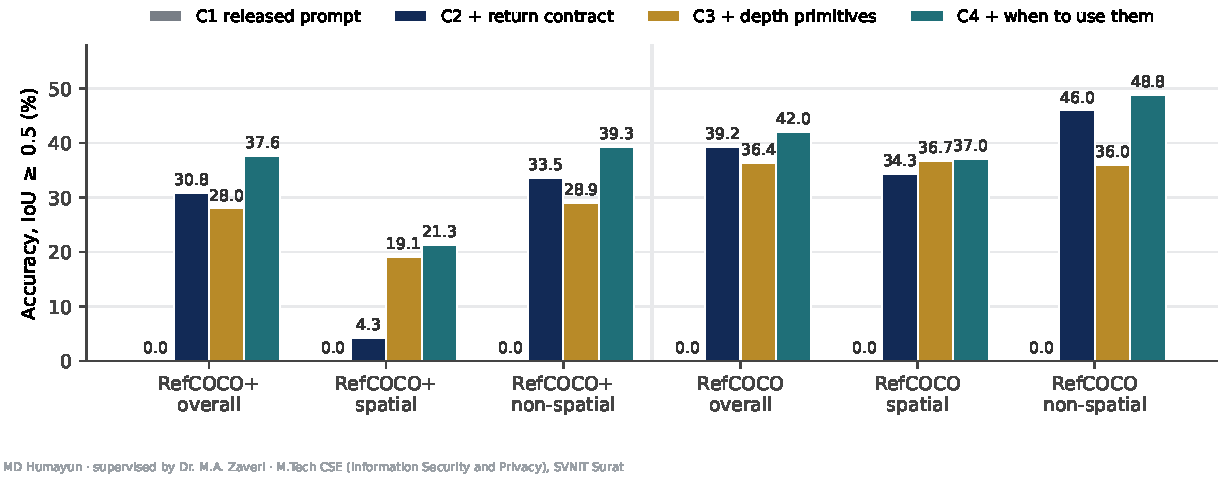
\includegraphics[width=\textwidth]{results/figures/fig1_main_result.pdf}
\caption{Accuracy at IoU $\geq0.5$ for all four prompt conditions, both datasets,
split by subset. $n=500$ per bar. C1 is the released prompt; C2 adds the return-type
contract; C3 adds depth primitives; C4 adds a rule for when they apply. The three
rightmost groups act as controls: a method that improved only its target subset would
be a trade rather than a gain.}
\label{fig:main}
\end{figure}

\textbf{The zero is not a crash} (Figure~\ref{fig:failure}). Of 500 baseline programs on RefCOCO, 336 executed
to completion and returned a \emph{string}; none returned a patch. Grounding is
scored by IoU against a box, so a sentence cannot score however correct its English.
Missing modules were ruled out as a cause: \texttt{simple\_query} and
\texttt{llm\_query} are given neutral empty-string fallbacks (D10) so that no program
can fail for lack of a module we chose not to load. That concession strictly favours
the baseline and does not change its score.

\begin{figure}[htbp]\centering
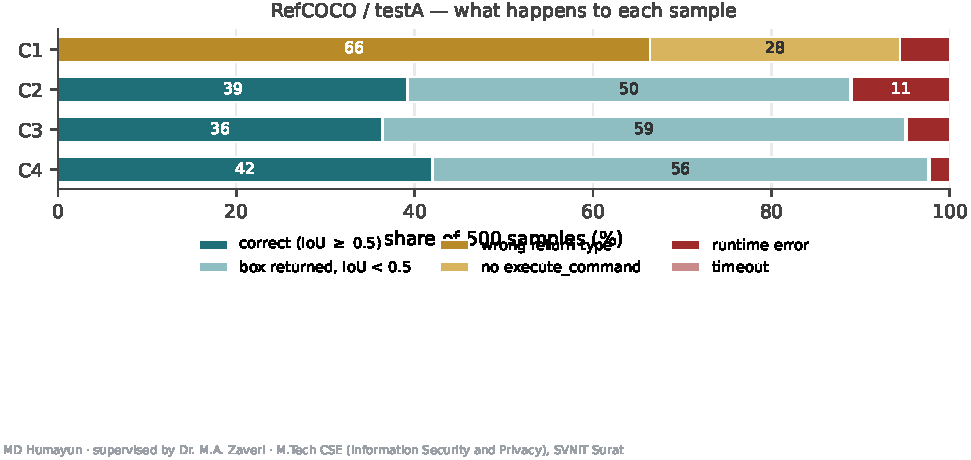
\includegraphics[width=\textwidth]{results/figures/fig7_failure_modes.pdf}
\caption{Every sample classified by what happened to it, RefCOCO/testA. C1 fails on
\emph{return type} --- it never reaches localisation. By C4 those categories are gone
and the residual failure is a localisation miss, which is a perception limit rather
than a specification bug. An accuracy figure alone conflates the two.}
\label{fig:failure}
\end{figure}

\textbf{A second, unanticipated effect.} Under the released prompt many generations
never defined \texttt{execute\_command} at all --- the model emitted prose or
malformed markdown: 136/500 (27.2\%) on RefCOCO and 214/500 (42.8\%) on RefCOCO+,
against zero under the contract. The contract disciplines output \emph{format} as
well as return type; these are separable failures and are reported separately.

\textbf{Robustness.} Greedy decoding is deterministic, so variance was estimated by
sampling ($T{=}0.7$, seeds 1--3, RefCOCO, $n{=}500$): $36.07 \pm 1.75$ against
$39.20$ greedy. Greedy beats all three sampled seeds, as expected when one program
shape is correct.

% =====================================================================
\section{Result 2 — the spatial gap, and what it is made of}

With the contract in place, accuracy splits by subset (relational-term lexicon):

\begin{table}[htbp]\centering\small
\caption{Spatial breakdown, grounding-contract condition. The baseline scores 0
everywhere and is omitted.}
\label{tab:spatial}
\begin{tabular}{@{}llrrr@{}}
\toprule
\textbf{Dataset} & \textbf{Subset} & \textbf{n} & \textbf{Accuracy} & \textbf{Mean IoU} \\
\midrule
RefCOCO  & spatial     & 289 & 35.29\% & 0.3475 \\
RefCOCO  & non-spatial & 211 & 44.55\% & 0.4378 \\
RefCOCO+ & spatial     & 47  & \down{6.38\%} & 0.1037 \\
RefCOCO+ & non-spatial & 453 & 34.44\% & 0.3474 \\
\bottomrule
\end{tabular}
\end{table}

\textbf{The gap is not a capacity problem} (Figure~\ref{fig:scale}). Repeating the whole pipeline with
Qwen2.5-Coder at 1.5B, 7B and 32B, greedy, same prompts and same perception stack:

\begin{center}\small
\begin{tabular}{@{}lrrrr@{}}
\toprule
\textbf{Generator} & \textbf{Baseline} & \textbf{+ Contract} & \textbf{spatial} & \textbf{non-spatial} \\
\midrule
1.5B & 0.80\% & 34.40\% & 34.95\% & 33.65\% \\
7B   & 0.00\% & 39.20\% & 35.29\% & 44.55\% \\
32B  & 0.00\% & 40.80\% & 34.95\% & 48.82\% \\
\bottomrule
\end{tabular}
\end{center}

\vspace{3pt}
\begin{figure}[htbp]\centering
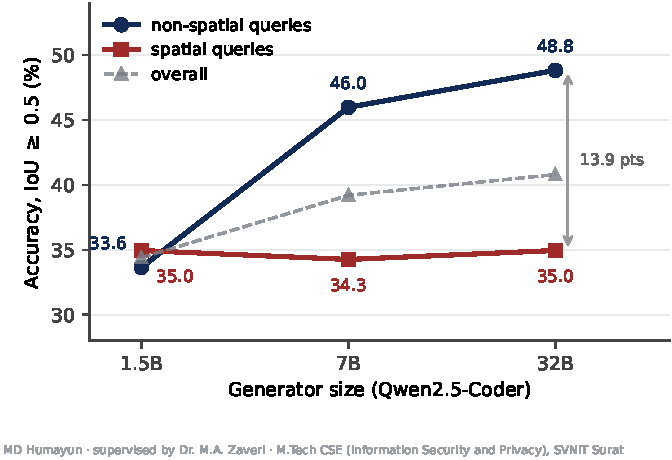
\includegraphics[width=0.62\textwidth]{results/figures/fig2_scale.pdf}
\caption{The same pipeline at three generator sizes, condition C2. Non-spatial
accuracy climbs with capacity; spatial accuracy does not move. Same images, same
detector, same prompt --- only the generator differs. This is the evidence that the
spatial deficit is an interface problem rather than a capacity one.}
\label{fig:scale}
\end{figure}

Two things follow. Result 1 is scale-independent: a 32B model still emits 87.6\%
task-invalid programs under the released prompt and still scores 0.00\%, and the same
three sentences repair it. Scaling 1.5B\,$\to$\,32B buys 6.4 accuracy points; the
prompt contract buys 33--41. More importantly, \textbf{spatial accuracy does not move
with scale at all} --- 34.95 / 35.29 / 34.95, with the smallest and largest models
identical to two decimal places --- while non-spatial accuracy rises by 15.2 points
on the same images with the same modules. A larger generator writes better programs
for everything except spatial relations, where it writes programs that are exactly as
wrong. If the spatial deficit were a program-synthesis problem, capacity would help;
it demonstrably does elsewhere. The bottleneck is the interface.

We expected the gap to \emph{shrink} on RefCOCO+, since that dataset forbids spatial
relations. It widened threefold. A manual audit of all 47 RefCOCO+ spatial queries
explains why: the two subsets contain \textbf{different kinds of spatial language}.

\begin{center}\small
\begin{tabular}{@{}p{0.16\textwidth}p{0.36\textwidth}p{0.40\textwidth}@{}}
\toprule
 & \textbf{RefCOCO} & \textbf{RefCOCO+} \\
\midrule
Type & 2D image-plane & depth and inter-object \\
Examples & \emph{man on right}, \emph{person bottom left} & \emph{man closest to us},
\emph{farthest man}, \emph{umpire behind catcher} \\
Resolvable by & sorting patch coordinates in base Python & requires
\texttt{compute\_depth} or 3D geometry \\
Accuracy & 35.29\% & 6.38\% \\
\bottomrule
\end{tabular}
\end{center}

\vspace{4pt}
Forbidding spatial language removed viewer-frame \emph{directional} expressions and
left depth-ordering and relational ones. The released prompt's instruction to use
base Python for ``left/right/up/down'' works for the first and cannot work for the
second. Consistently, Milestone 1 found \texttt{compute\_depth} invoked 29 times
against 547 for \texttt{find} and 5 for \texttt{distance}: the geometric API is
effectively unused, by design of the prompt.

Two further observations support this reading. All three successes in the RefCOCO+
spatial subset are depth queries with very high IoU (0.97, 0.96, 0.92) --- when depth
ordering \emph{is} attempted correctly, localisation is excellent; it is usually not
attempted. And across seeds, spatial variance is roughly four times non-spatial
variance ($\pm3.35$ vs $\pm0.72$): programs handling spatial relations are not merely
less accurate but less \emph{stable}, sometimes resolving a relation by sorting and
sometimes dropping it entirely.

\textbf{Caveat.} $n{=}47$, so 6.38\% is 3 of 47 and the interval is wide. The lexicon
also produces roughly five false positives in that subset, which would push true
depth-query accuracy lower still. The direction is informative; the value is not.

% =====================================================================
\section{Reproducibility record}

\begin{center}\small
\begin{tabular}{@{}p{0.05\textwidth}p{0.30\textwidth}p{0.57\textwidth}@{}}
\toprule
\textbf{ID} & \textbf{Deviation} & \textbf{Reason / effect} \\
\midrule
D1 & Codex $\rightarrow$ Qwen2.5-Coder-7B & Codex retired; no faithful option. The
substitution is what exposes Result 1, and is the dominant term in the gap to 72.0. \\
D2 & Scope: grounding only & GQA/OK-VQA/NExT-QA need $\sim$250\,GB against 231\,GB
quota; OK-VQA also needs GPT-3, likewise retired. \\
D3 & RefCOCO annotations from Internet Archive & The canonical UNC host no longer
resolves. Archived zips are byte-identical. No effect. \\
D5, D6 & GLIP built for sm\_90 & CUDA 11.6 has no sm\_90. Headers and NumPy aliases
updated; kernels unchanged. Verified numerically. \\
D8 & GLIP threshold $0.2$ (paper unspecified) & Swept on 20 samples: 0.5 loses 8/20
detections, 0.2 gives mean IoU 0.776. Material and under-validated. \\
D9 & X-VLM $\rightarrow$ CLIP & X-VLM weights are Google-Drive-only. CLIP scores
globally, so attribute checks are weaker --- costliest on RefCOCO+. \\
D10 & \texttt{simple\_query}/\texttt{llm\_query} return \texttt{""} & Loading
BLIP-2-XXL and an 8B text LLM is out of scope. Favours the baseline; no effect on the
contract condition. \\
\bottomrule
\end{tabular}
\end{center}

\vspace{4pt}
\textbf{Two recorded failures.} A first hypothesis --- that spatial queries would
collapse into a single opaque \texttt{simple\_query} call, as the paper's GQA prompt
instructs --- was tested and rejected (collapse rate $\approx0\%$); that instruction
applies to GQA, and grounding cannot use \texttt{simple\_query} because it must
return a patch. Separately, an early 500-sample execution ran on a login node with no
GPU, producing a complete and entirely fake results table; those runs were deleted
and job scripts now assert \texttt{torch.cuda.is\_available()}. Silent CPU fallback
is the most dangerous failure mode encountered, because it yields plausible output
rather than an error.

\textbf{Artefacts.} Every run writes a timestamped directory with resolved config,
per-query programs, per-sample records and a summary; SLURM job IDs are recorded;
\texttt{docs/research\_log.md} (540+ lines) documents the full arc including failures.

% =====================================================================
\section{Where the gap to 72.0 comes from}

\begin{figure}[htbp]\centering
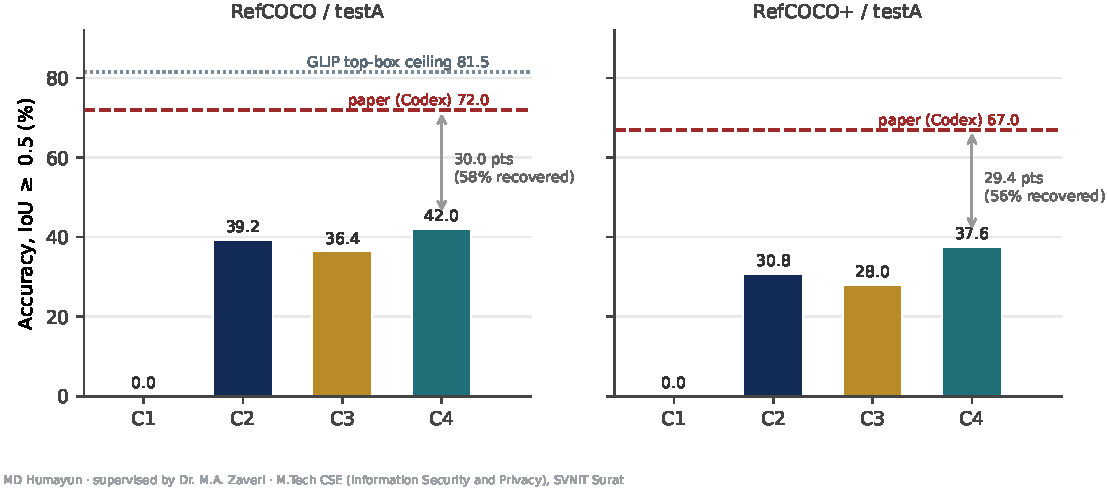
\includegraphics[width=\textwidth]{results/figures/fig10_vs_paper.pdf}
\caption{Reproduced against reported. The dotted line is GLIP alone taking its single
best box (81.5\%, $n=200$ held out) --- \emph{above} the paper's 72.0. Perception is
therefore not what separates this reproduction from the original. No decomposition of
the gap into individual deviations is shown: those ablations were not run, and
inventing the split would be fabrication.}
\label{fig:vspaper}
\end{figure}

C4 reaches 42.00 on RefCOCO against a reported 72.0. Raw GLIP top-box accuracy on this data is
78.9\%, so perception caps the system near 79\% before any program runs; program-level
selection loses roughly 40 points from there. Ordered by likely size, the
contributors are D1 (generator substitution, dominant), the perception ceiling,
D9 (X-VLM$\rightarrow$CLIP, costliest on RefCOCO+, consistent with 31.80 vs 39.20),
and D8 (threshold tuned on 20 samples). No claim of a faithful reproduction is made:
what is reproduced is the method; what is measured is what happens to it when its
generator is replaced.

% =====================================================================
\section{Milestone 3 --- a depth-grounded API}

The API exposes \texttt{compute\_depth()}: one scalar, the median relative depth of a
patch. That can express ``A is behind B'' but not ``the third closest'', ``between A
and B in depth'', or any ordering over more than two objects. The prompt also directs
the generator to use base Python for ``left/right/up/down'', and it complies --- over
500 programs, \texttt{find} is called 547 times and \texttt{compute\_depth} 29.

We added \texttt{depth\_order}, \texttt{is\_behind}, \texttt{is\_in\_front\_of},
\texttt{is\_between\_3d} and \texttt{distance\_3d} to \texttt{ImagePatch}, and wrote
two further prompt variants: C3 documents the primitives, C4 additionally states when
they apply and when they do not.

\subsection{Two prerequisites, both of which were broken}

\textbf{The depth sign was inverted.} The shipped wrapper returned raw MiDaS output.
MiDaS predicts \emph{inverse} depth: larger means \emph{closer}. Every comparison
built on \texttt{compute\_depth()} therefore ran backwards relative to its own
docstring. The sign was settled by removing both the detector and any synthetic data
--- take RefCOCO+ depth queries, use \textbf{ground-truth boxes only}, and ask
whether the annotated target sits at the correct end of the ordering:

\begin{center}\small
\begin{tabular}{@{}lr@{}}
\toprule
 & \textbf{correct} \\
\midrule
without inversion & 2/25 = \down{8\%} \\
with inversion & 20/25 = \up{80\%} \\
chance (3.8 objects/image) & 26\% \\
\bottomrule
\end{tabular}
\end{center}

\vspace{3pt}
8\% is far \emph{below} chance --- the signature of a systematically inverted signal,
not a weak one. A synthetic test scene had earlier indicated the opposite and cost
several hours: it was a brightness gradient the model read as depth. \textbf{Synthetic
scenes are unreliable for validating perceptual signals.} The ordering semantics are
now pinned by 18 unit-test assertions so the sign cannot silently flip again.

\textbf{The generator had to actually use the API.} The risk that it would ignore the
new primitives as it ignores \texttt{compute\_depth} did not materialise:

\begin{center}\small
\begin{tabular}{@{}lrrrr@{}}
\toprule
\textbf{Condition} & \texttt{find} & \texttt{compute\_depth} & \texttt{depth\_order} & \textbf{other prims} \\
\midrule
C2 & 639 & 23 & 0 & 0 \\
C3 & 598 & 19 & 119 & 63 \\
C4 & 559 & --- & 37 & 7 \\
\bottomrule
\end{tabular}
\end{center}

\vspace{3pt}
Zero adoption under the older prompts, strong adoption once offered. Under C4 the
count falls to 37 --- RefCOCO contains few depth queries, so that is the routing rule
working, not the primitives being abandoned. On RefCOCO+, which has 47 depth-word
queries, C4 makes 33 \texttt{depth\_order} calls.

\subsection{Result}

\begin{figure}[htbp]\centering
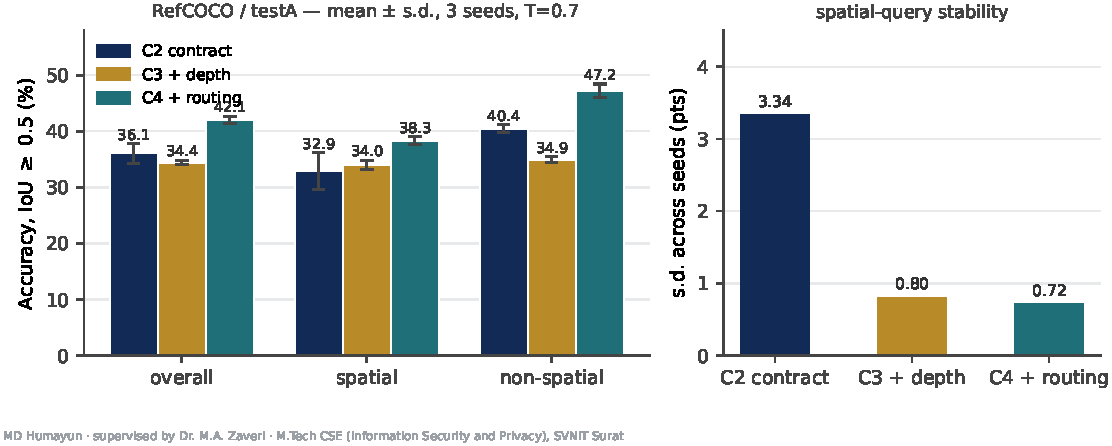
\includegraphics[width=\textwidth]{results/figures/fig6_seed_variance.pdf}
\caption{Seed variance, sampling at $T{=}0.7$. Left: C4 separates from C2 by 6.0
points against standard deviations under 2. Note that C2's greedy result (39.20) sits
1.8 s.d.\ \emph{above} its own sampled mean, so the greedy table understates the
difference. Right: standard deviation on spatial queries alone. The explicit
primitive removes the improvisation the generator otherwise performs afresh on every
sample, and the variance falls 4.6$\times$.}
\label{fig:seeds}
\end{figure}

\begin{table}[htbp]\centering\small
\caption{Accuracy at IoU $\geq0.5$, Qwen2.5-Coder-7B, greedy, $n=500$ per cell.
C3 offers the depth primitives; C4 also states when to use them.}
\label{tab:m3}
\begin{tabular}{@{}llrrrr@{}}
\toprule
\textbf{Dataset} & \textbf{Subset} & \textbf{C1} & \textbf{C2} & \textbf{C3} & \textbf{C4} \\
\midrule
RefCOCO+ & overall & 0.00 & 30.80 & 28.00 & \up{37.60} \\
RefCOCO+ & spatial ($n{=}47$) & 0.00 & 4.26 & 19.15 & \up{21.28} \\
RefCOCO+ & non-spatial & 0.00 & 33.55 & \down{28.92} & \up{39.29} \\
\midrule
RefCOCO & overall & 0.00 & 39.20 & 36.40 & \up{42.00} \\
RefCOCO & spatial ($n{=}289$) & 0.00 & 34.26 & 36.68 & \up{37.02} \\
RefCOCO & non-spatial ($n{=}211$) & 0.00 & 45.97 & \down{36.02} & \up{48.82} \\
\bottomrule
\end{tabular}
\end{table}

\textbf{C3 wins the target subset and loses elsewhere.} Depth-word queries go
4.26\,$\to$\,19.15, but non-spatial accuracy falls 45.97\,$\to$\,36.02 on RefCOCO and
33.55\,$\to$\,28.92 on RefCOCO+, so overall accuracy drops. \texttt{depth\_order} is
invoked 119 times on RefCOCO, where most queries need no depth at all: \emph{given a
new primitive, the generator reaches for it indiscriminately}.

\textbf{C4 changes one thing} (Figures~\ref{fig:seeds} and~\ref{fig:qual}) --- three sentences stating that the depth functions
apply only to depth relations, plus two examples of queries that should \emph{not}
use them --- \textbf{and beats C2 in every cell of both datasets}. The depth gain
survives (21.28) while non-spatial rises above C2 as well (48.82 against 45.97),
presumably because the negative examples also clarify the 2D and attribute paths.

\begin{figure}[htbp]\centering
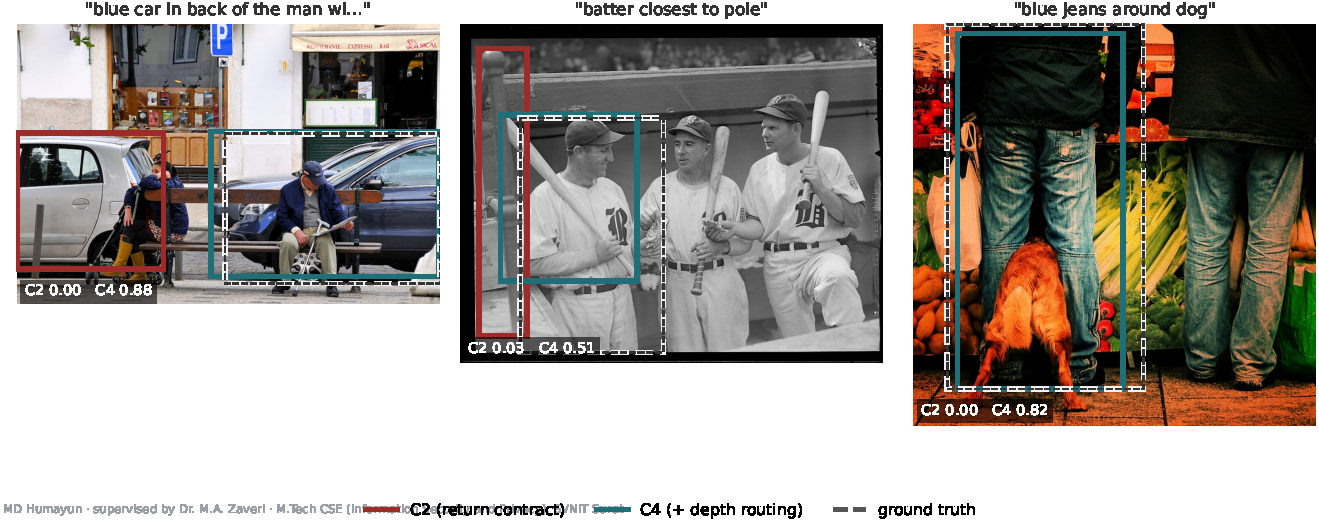
\includegraphics[width=\textwidth]{results/figures/fig4_qualitative.pdf}
\caption{Depth queries where C4 succeeds and C2 fails. Red: C2's prediction. Teal:
C4's. Dashed: ground truth. The failures are not near-misses --- without a primitive
for ``closest'', the program selects a different object entirely.}
\label{fig:qual}
\end{figure}

This is the sharper finding of Milestone 3. Providing a capability is not sufficient;
the specification must also delimit \emph{when} it applies. That is the same class of
omission as Result~1, where the released prompt failed to state the return type.

\subsection{A compute artefact, found and removed}

RefCOCO+ under C4 initially showed 40 timeouts at the 60\,s executor limit. The
programs do not loop --- they call \texttt{verify\_property} on every candidate:

\begin{lstlisting}
black = [p for p in person_patches if p.verify_property("person", "black shirt")]
\end{lstlisting}

\vspace{-3pt}
At threshold 0.2 \texttt{find} returns $\approx$40 boxes, so that is $\approx$40 CLIP
forward passes. The cause is C4's own routing rule, which directs attribute queries to
\texttt{verify\_property} on an attribute-based dataset: the instruction is correct
and it exposed a bottleneck. All three RefCOCO+ conditions were re-run at 300\,s;
C2 and C3 were unchanged, confirming the earlier C4 figure had been a lower bound
(35.40\,$\to$\,37.60).

Execution robustness improves monotonically across conditions --- RefCOCO errors
55\,$\to$\,24\,$\to$\,11 and patch returns 444\,$\to$\,475\,$\to$\,488 for
C2\,$\to$\,C3\,$\to$\,C4 --- consistent with more worked examples disciplining
generation generally.


\subsection{A 15-point result that was not ours}

The detection threshold returns roughly 20 candidates per image (Appendix,
Figure~8). Capping \texttt{find} to $k$ of them, on the \emph{same} C4 programs:

\begin{center}\small
\begin{tabular}{@{}lrrr@{}}
\toprule
\textbf{cap} & \textbf{overall} & \textbf{spatial} & \textbf{non-spatial} \\
\midrule
off & 42.80 & 37.72 & 49.76 \\
$k=12$ & 45.20 & 41.52 & 50.24 \\
$k=6$ & 49.60 & 47.75 & 52.13 \\
$k=3$ & \textbf{57.60} & \textbf{61.59} & 52.13 \\
\bottomrule
\end{tabular}
\end{center}

\vspace{3pt}
57.60\% would be the best figure in this project by fifteen points, and 61.59\% on
spatial queries would exceed every non-spatial result. It is not reportable, and the
control is why.

Applying the identical cap to \textbf{C2}, which contains no depth primitives at all:

\begin{center}\small
\begin{tabular}{@{}lrrr@{}}
\toprule
 & \textbf{no cap} & \textbf{$k=3$} & \textbf{gain} \\
\midrule
C2 spatial & 34.60 & 57.09 & \down{$+22.5$} \\
C4 spatial & 37.72 & 61.59 & $+23.9$ \\
C2 non-spatial & 45.02 & 45.50 & $+0.5$ \\
C4 non-spatial & 49.76 & 52.13 & $+2.4$ \\
\bottomrule
\end{tabular}
\end{center}

\vspace{3pt}
C2's spatial accuracy rises 22.5 points from the cap alone, with no depth reasoning
anywhere in the pipeline. Of C4's 23.9, roughly 1.4 points are attributable to depth
and the rest to the candidate set.

\textbf{The mechanism is mechanical.} Choosing among three candidates rather than
twenty raises the hit rate by construction --- random selection alone scores 33\% at
$k{=}3$ against 5\% at $k{=}20$ --- and in RefCOCO the referred object is almost
always among the most confident detections. That non-spatial queries gain almost
nothing ($+0.5$ for C2) confirms it: those queries verify attributes rather than
selecting among same-class candidates, so a smaller set does not help them. Only
``pick one of $N$ people'' benefits, and it benefits however the pick is made.

\textbf{Decision.} \texttt{max\_detections} remains disabled for every reported
number. Enabling it and reporting 57.60\% would exploit a property of the dataset
rather than demonstrate a method. NMS is likewise left off: it helps RefCOCO
marginally (42.00\,$\to$\,42.80) but harms RefCOCO+ depth queries badly
(21.28\,$\to$\,12.77), because suppressing overlapping boxes removes exactly the
depth-distinct instances a depth query must tell apart.

\textbf{What survives.} C4's advantage over C2 holds under both settings --- 3.8
points uncapped, 5.4 capped --- so the contribution does not rest on the cap.

This is the second occasion on which a tuned knob produced a large apparent gain that
dissolved under a control, the first being the depth sign, where a synthetic test
scene gave the wrong answer. Both were caught before anything was claimed, which is
the argument for running the control before writing the number down.

\subsection{What is claimed, and what is not}

Depth is claimed only as \emph{ordering}. COCO ships no camera intrinsics, so metric
distances would rest on an assumed field of view; \texttt{depth\_order} and
\texttt{is\_behind} need only monotonicity in true distance, which relative depth
provides once the sign is right. The depth subset is $n{=}47$, so 21.28\% carries a
wide interval --- the direction is established, the value is not. C3 and C4 are
single-seed.

\section{Limitations and next steps}

\begin{enumerate}[leftmargin=1.3em, itemsep=2pt]
\item Depth-subset results rest on $n{=}47$ queries ($n{=}25$ for the sign test).
Directions are clear; the values carry wide intervals. C3 and C4 are single-seed.
\item The GLIP threshold was re-swept on a held-out slice ($n{=}200$, samples
200--399): 0.2 is within 1.0 point of optimal for detection, so no reported number
changes --- but it is the wrong operating point for candidate \emph{selection}, as
Milestone 3 shows.
\item X-VLM substituted by CLIP (D9); the substitution most likely to be costing
accuracy, especially on RefCOCO+, and the source of the per-candidate compute cost
that produced the C4 timeouts.
\item \texttt{find} returns $\approx$40 candidates at the tuned threshold. That is
correct for top-box detection and wrong for any program that must select among
candidates --- it affects depth ordering and attribute checking alike. A
\texttt{max\_detections} knob exists but is disabled by default so that no reported
number depends on it (D12).
\item Seed variance measured on RefCOCO only ($36.07 \pm 1.75$ at $T{=}0.7$ against
39.20 greedy), and by sampling rather than retraining --- the standard caveat for a
decoding-only estimate. Spatial variance is four times non-spatial variance
($\pm3.35$ vs $\pm0.72$): spatial programs are less stable, not merely less accurate.
\item Spatial subsets are identified by lexicon, not human annotation.
\end{enumerate}


\clearpage
\appendix
\section{Supporting figures}

The six figures below are not needed to follow the argument, but each answers a
question a careful reader will ask. All regenerate with
\texttt{python make\_figures.py --qual}.

\begin{figure}[htbp]\centering
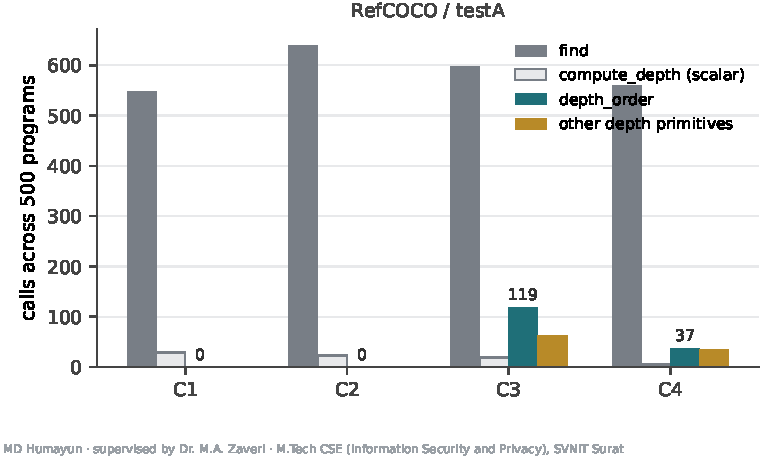
\includegraphics[width=0.68\textwidth]{results/figures/fig3_api_adoption.pdf}
\caption{\textbf{API adoption.} Occurrences of each API call across 500 generated
programs, RefCOCO/testA. \emph{Did the generator use the new API, or ignore it?} This
was the main risk: ViperGPT already exposes \texttt{compute\_depth}, and the generator
calls it 29 times against 547 for \texttt{find}. Under C3 \texttt{depth\_order} is
called 119 times, under C1 and C2 zero times. Under C4 it falls to 37 --- the routing
rule working, not the primitive being abandoned, since RefCOCO contains few depth
queries. On RefCOCO+, which has 47, C4 makes 33 calls.}
\end{figure}

\begin{figure}[htbp]\centering
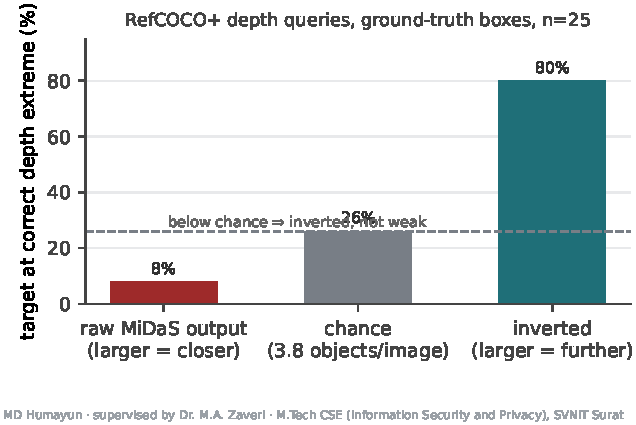
\includegraphics[width=0.56\textwidth]{results/figures/fig9_depth_sign.pdf}
\caption{\textbf{Depth sign validation.} RefCOCO+ depth queries scored against
ground-truth boxes, no detector involved. \emph{Is the depth signal real, and is its
sign right?} MiDaS predicts \emph{inverse} depth --- larger means closer --- and the
original wrapper returned it unmodified, so every comparison ran backwards. The tell
is that 8\% is \emph{below} the 26\% chance level: a weak signal scores near chance,
an inverted one scores below it. A synthetic test scene had earlier indicated no
inversion was needed and cost several hours; it was a brightness gradient the model
read as depth. Synthetic scenes are unreliable for validating perceptual signals.}
\end{figure}

\begin{figure}[htbp]\centering
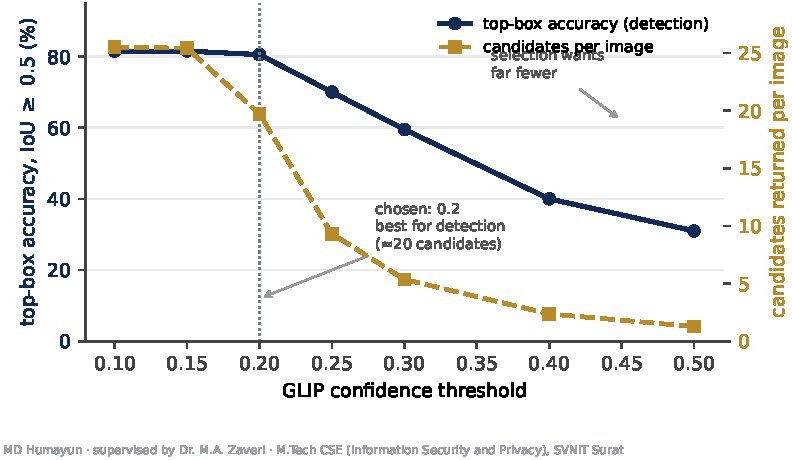
\includegraphics[width=0.62\textwidth]{results/figures/fig8_threshold_tradeoff.pdf}
\caption{\textbf{One threshold, two incompatible jobs.} \emph{Is the detection
threshold well chosen?} It is --- for detection. At 0.2, top-box accuracy peaks at
81.5\%, validated on a held-out slice ($n=200$, disjoint from every reported cell).
But it also returns $\approx$20 candidates per image, and any program that must
\emph{select} among them --- depth ordering, per-candidate attribute checking --- wants
far fewer. The same knob cannot serve both. A \texttt{max\_detections} control exists
but is disabled by default so that no reported number depends on it (D12).}
\end{figure}

\begin{figure}[htbp]\centering
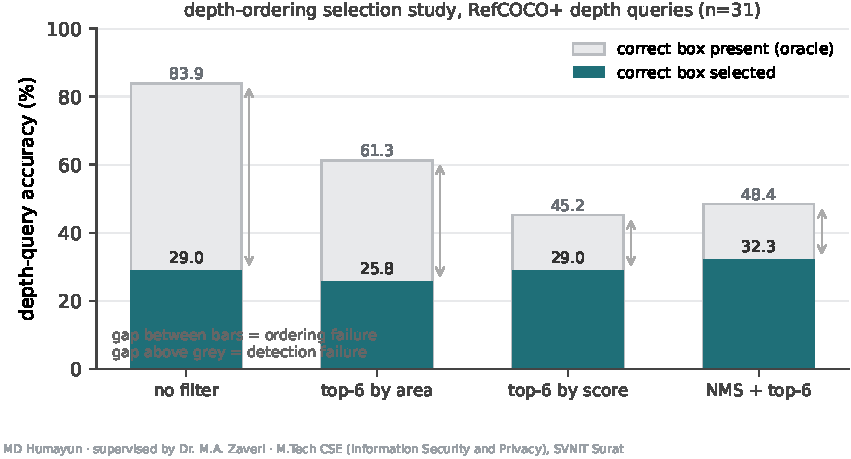
\includegraphics[width=0.68\textwidth]{results/figures/fig12_headroom.pdf}
\caption{\textbf{Achieved against achievable.} Depth-ordering selection study. Grey:
the correct box was present among the candidates. Teal: it was selected. The gap
between bars is an ordering failure; the gap from grey to 100\% is a detection
failure. On the unfiltered set the correct box is present 83.9\% of the time and
selected 29.0\%; filtering to six candidates costs oracle but converts far better,
reaching 32.3\% against 48.4\% achievable. The binding constraint has moved from
ordering to detection, which is where further work should go.}
\end{figure}

\begin{figure}[htbp]\centering
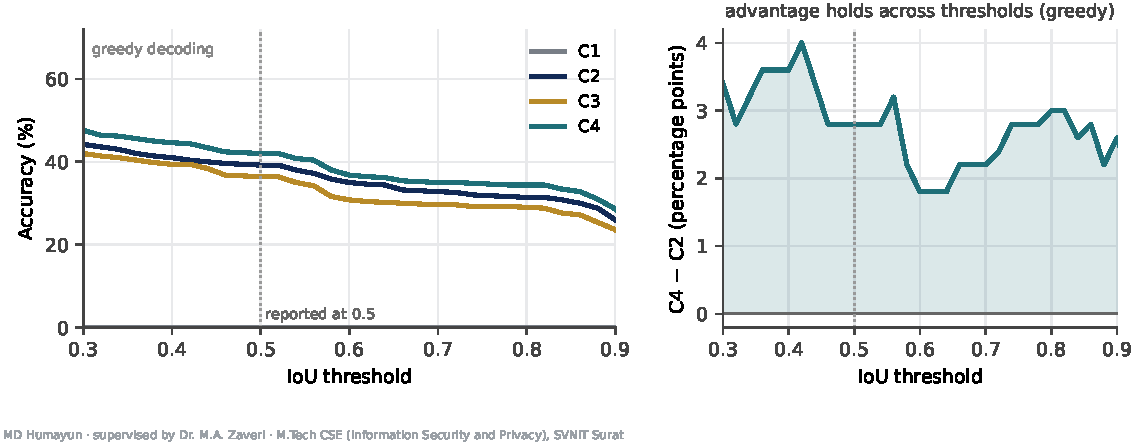
\includegraphics[width=\textwidth]{results/figures/fig11_iou_sweep.pdf}
\caption{\textbf{IoU threshold sensitivity.} \emph{Is the result an artefact of
scoring at IoU 0.5?} No. The threshold is used because the paper uses it, but the
C4 advantage stays positive across 0.3--0.9 (1.8 to 4.0 points under greedy). Were the
advantage confined to the neighbourhood of 0.5, it would suggest the conditions differ
in box tightness rather than in object selection.}
\end{figure}

\begin{figure}[htbp]\centering
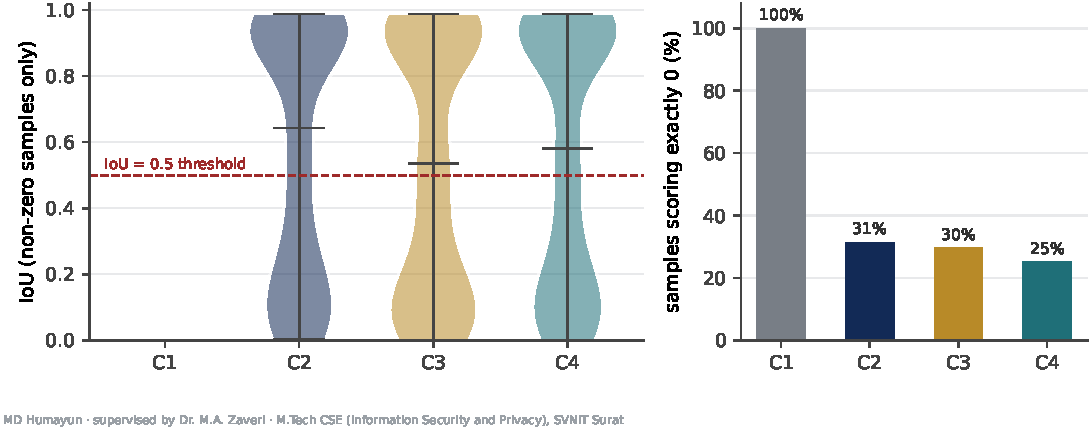
\includegraphics[width=\textwidth]{results/figures/fig5_iou_distribution.pdf}
\caption{\textbf{IoU distribution.} \emph{Does the mean come from a few good cases or
many mediocre ones?} The distributions are strongly bimodal --- programs either
localise well (IoU above 0.8) or miss entirely, with little middle ground. That is
what one expects when the failure mode is selecting the wrong object rather than
drawing a loose box. The right panel restates the headline in a different currency:
the share of samples scoring nothing at all falls from 100\% to 25\%.}
\end{figure}

\begin{figure}[htbp]\centering
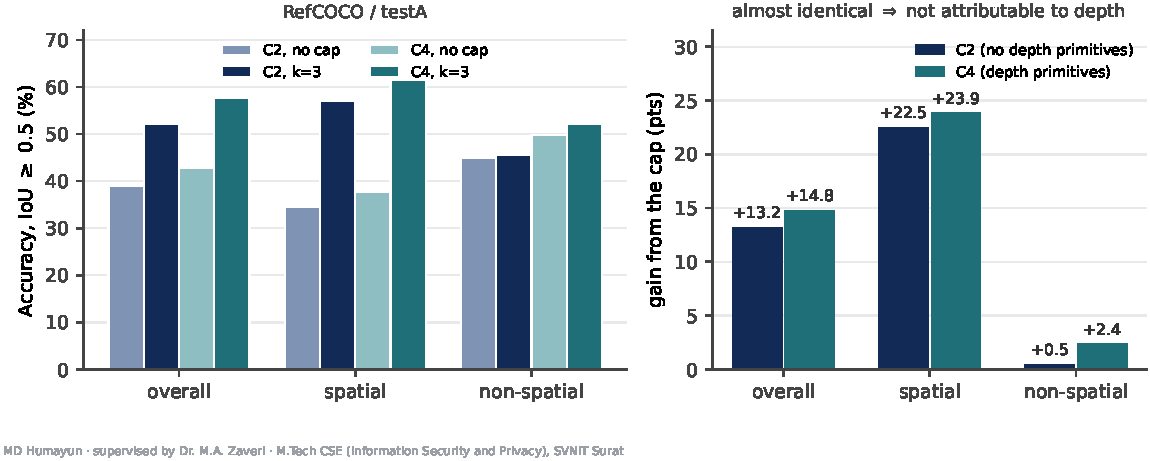
\includegraphics[width=\textwidth]{results/figures/fig13_cap_control.pdf}
\caption{\textbf{The control that disqualified a 15-point result.} Left: both
conditions with and without a three-candidate cap. Right: the gain the cap alone
provides, by subset. C2 has no depth primitives and gains almost exactly what C4
gains, so the improvement belongs to the candidate set rather than to depth
reasoning. Non-spatial queries barely move, which identifies the mechanism.}
\end{figure}

\section{What the figures do not show}

Stated explicitly, because absence is easy to mistake for oversight.

\begin{itemize}[leftmargin=1.3em, itemsep=3pt]
\item \textbf{No decomposition of the gap to the paper.} Attributing points to D1
(Codex), D9 (X-VLM) or D8 (threshold) individually would require ablations that were
not run.
\item \textbf{No per-depth-word breakdown.} \emph{closest}, \emph{farthest} and
\emph{behind} occur a handful of times each within the 47-query subset; a chart at
that resolution would be noise.
\item \textbf{Depth-subset intervals are wide.} $n=47$: the direction of the
4.26\,$\to$\,21.28 result is established, the exact value is not.
\item \textbf{C3 and C4 seeds cover RefCOCO only.} RefCOCO+ figures are single-run.
\end{itemize}

\vspace{8pt}\hrule\vspace{3pt}
{\footnotesize\color{midgrey}
All figures traceable to a run directory, an archived summary in
\texttt{results/m2\_summaries/}, and a SLURM job ID. Milestone 1: jobs 29187, 29193.
Milestone 2: jobs 29290, 29292, 29301, 29306, 29318, 29321, 29352, 29404. Milestone 3: jobs 29459, 29523, 29524, 29525. Repository tags
\texttt{m1-complete}, \texttt{m2-glip-verified}, \texttt{m2-execution},
\texttt{m2-complete}, \texttt{m3-depth-api}, \texttt{m3-final}.}

\end{document}
